\PassOptionsToPackage{unicode=true}{hyperref} % options for packages loaded elsewhere
\PassOptionsToPackage{hyphens}{url}
%
\documentclass[]{book}
\usepackage{lmodern}
\usepackage{amssymb,amsmath}
\usepackage{ifxetex,ifluatex}
\usepackage{fixltx2e} % provides \textsubscript
\ifnum 0\ifxetex 1\fi\ifluatex 1\fi=0 % if pdftex
  \usepackage[T1]{fontenc}
  \usepackage[utf8]{inputenc}
  \usepackage{textcomp} % provides euro and other symbols
\else % if luatex or xelatex
  \usepackage{unicode-math}
  \defaultfontfeatures{Ligatures=TeX,Scale=MatchLowercase}
\fi
% use upquote if available, for straight quotes in verbatim environments
\IfFileExists{upquote.sty}{\usepackage{upquote}}{}
% use microtype if available
\IfFileExists{microtype.sty}{%
\usepackage[]{microtype}
\UseMicrotypeSet[protrusion]{basicmath} % disable protrusion for tt fonts
}{}
\IfFileExists{parskip.sty}{%
\usepackage{parskip}
}{% else
\setlength{\parindent}{0pt}
\setlength{\parskip}{6pt plus 2pt minus 1pt}
}
\usepackage{hyperref}
\hypersetup{
            pdftitle={Statistics with R},
            pdfauthor={Hugo Quené},
            pdfborder={0 0 0},
            breaklinks=true}
\urlstyle{same}  % don't use monospace font for urls
\usepackage{color}
\usepackage{fancyvrb}
\newcommand{\VerbBar}{|}
\newcommand{\VERB}{\Verb[commandchars=\\\{\}]}
\DefineVerbatimEnvironment{Highlighting}{Verbatim}{commandchars=\\\{\}}
% Add ',fontsize=\small' for more characters per line
\usepackage{framed}
\definecolor{shadecolor}{RGB}{248,248,248}
\newenvironment{Shaded}{\begin{snugshade}}{\end{snugshade}}
\newcommand{\AlertTok}[1]{\textcolor[rgb]{0.94,0.16,0.16}{#1}}
\newcommand{\AnnotationTok}[1]{\textcolor[rgb]{0.56,0.35,0.01}{\textbf{\textit{#1}}}}
\newcommand{\AttributeTok}[1]{\textcolor[rgb]{0.77,0.63,0.00}{#1}}
\newcommand{\BaseNTok}[1]{\textcolor[rgb]{0.00,0.00,0.81}{#1}}
\newcommand{\BuiltInTok}[1]{#1}
\newcommand{\CharTok}[1]{\textcolor[rgb]{0.31,0.60,0.02}{#1}}
\newcommand{\CommentTok}[1]{\textcolor[rgb]{0.56,0.35,0.01}{\textit{#1}}}
\newcommand{\CommentVarTok}[1]{\textcolor[rgb]{0.56,0.35,0.01}{\textbf{\textit{#1}}}}
\newcommand{\ConstantTok}[1]{\textcolor[rgb]{0.00,0.00,0.00}{#1}}
\newcommand{\ControlFlowTok}[1]{\textcolor[rgb]{0.13,0.29,0.53}{\textbf{#1}}}
\newcommand{\DataTypeTok}[1]{\textcolor[rgb]{0.13,0.29,0.53}{#1}}
\newcommand{\DecValTok}[1]{\textcolor[rgb]{0.00,0.00,0.81}{#1}}
\newcommand{\DocumentationTok}[1]{\textcolor[rgb]{0.56,0.35,0.01}{\textbf{\textit{#1}}}}
\newcommand{\ErrorTok}[1]{\textcolor[rgb]{0.64,0.00,0.00}{\textbf{#1}}}
\newcommand{\ExtensionTok}[1]{#1}
\newcommand{\FloatTok}[1]{\textcolor[rgb]{0.00,0.00,0.81}{#1}}
\newcommand{\FunctionTok}[1]{\textcolor[rgb]{0.00,0.00,0.00}{#1}}
\newcommand{\ImportTok}[1]{#1}
\newcommand{\InformationTok}[1]{\textcolor[rgb]{0.56,0.35,0.01}{\textbf{\textit{#1}}}}
\newcommand{\KeywordTok}[1]{\textcolor[rgb]{0.13,0.29,0.53}{\textbf{#1}}}
\newcommand{\NormalTok}[1]{#1}
\newcommand{\OperatorTok}[1]{\textcolor[rgb]{0.81,0.36,0.00}{\textbf{#1}}}
\newcommand{\OtherTok}[1]{\textcolor[rgb]{0.56,0.35,0.01}{#1}}
\newcommand{\PreprocessorTok}[1]{\textcolor[rgb]{0.56,0.35,0.01}{\textit{#1}}}
\newcommand{\RegionMarkerTok}[1]{#1}
\newcommand{\SpecialCharTok}[1]{\textcolor[rgb]{0.00,0.00,0.00}{#1}}
\newcommand{\SpecialStringTok}[1]{\textcolor[rgb]{0.31,0.60,0.02}{#1}}
\newcommand{\StringTok}[1]{\textcolor[rgb]{0.31,0.60,0.02}{#1}}
\newcommand{\VariableTok}[1]{\textcolor[rgb]{0.00,0.00,0.00}{#1}}
\newcommand{\VerbatimStringTok}[1]{\textcolor[rgb]{0.31,0.60,0.02}{#1}}
\newcommand{\WarningTok}[1]{\textcolor[rgb]{0.56,0.35,0.01}{\textbf{\textit{#1}}}}
\usepackage{longtable,booktabs}
% Fix footnotes in tables (requires footnote package)
\IfFileExists{footnote.sty}{\usepackage{footnote}\makesavenoteenv{longtable}}{}
\usepackage{graphicx,grffile}
\makeatletter
\def\maxwidth{\ifdim\Gin@nat@width>\linewidth\linewidth\else\Gin@nat@width\fi}
\def\maxheight{\ifdim\Gin@nat@height>\textheight\textheight\else\Gin@nat@height\fi}
\makeatother
% Scale images if necessary, so that they will not overflow the page
% margins by default, and it is still possible to overwrite the defaults
% using explicit options in \includegraphics[width, height, ...]{}
\setkeys{Gin}{width=\maxwidth,height=\maxheight,keepaspectratio}
\setlength{\emergencystretch}{3em}  % prevent overfull lines
\providecommand{\tightlist}{%
  \setlength{\itemsep}{0pt}\setlength{\parskip}{0pt}}
\setcounter{secnumdepth}{5}
% Redefines (sub)paragraphs to behave more like sections
\ifx\paragraph\undefined\else
\let\oldparagraph\paragraph
\renewcommand{\paragraph}[1]{\oldparagraph{#1}\mbox{}}
\fi
\ifx\subparagraph\undefined\else
\let\oldsubparagraph\subparagraph
\renewcommand{\subparagraph}[1]{\oldsubparagraph{#1}\mbox{}}
\fi

% set default figure placement to htbp
\makeatletter
\def\fps@figure{htbp}
\makeatother

\usepackage{booktabs}
\usepackage{amsthm}
\makeatletter
\def\thm@space@setup{%
  \thm@preskip=8pt plus 2pt minus 4pt
  \thm@postskip=\thm@preskip
}
\makeatother
\usepackage[]{natbib}
\bibliographystyle{apalike}

\title{Statistics with R}
\author{Hugo Quené}
\date{2020-04-11}

\begin{document}
\maketitle

{
\setcounter{tocdepth}{1}
\tableofcontents
}
\hypertarget{preface}{%
\chapter*{Preface}\label{preface}}
\addcontentsline{toc}{chapter}{Preface}

This booklet is written as accompaniment to the online tutorial on \emph{Statistics with R (Basics)}, to be held as part of the workshop on Experimental Methods in Language Acquisition Research (EMLAR, \url{https://emlar.wp.hum.uu.nl/}), Utrecht, on 17 April 2020.

Here's the abstract for the tutorial:

\begin{quote}
This tutorial will introduce the R programming environment for statistical analysis. Contrary to SPSS which is procedure-oriented (commands are verbs, e.g. ``compute''), R is object-oriented (objects are nouns, e.g. ``factor''). In this workshop, we will try to ease the learning curve of using R for your data analysis. Experience with statistical software is NOT required! We will use data simulation as well as real data sets, to explore topics like t-tests, \(\chi^2\) tests, and regression. We will also show how R produces publication-quality figures.
\end{quote}

This document is licensed under the \emph{GNU GPL 3} license (for details see
\url{https://www.gnu.org/licenses/gpl-3.0.en.html}). It was created with the \texttt{bookdown} package \citep{R-bookdown} in \href{https://www.rstudio.com}{Rstudio}.

Hugo Quené, Utrecht institute of Linguistics OTS, Utrecht University

\url{https://www.hugoquene.nl}

\hypertarget{ch:introduction}{%
\chapter{Introduction}\label{ch:introduction}}

This tutorial offers a first introduction into R.
R is available as freeware from
\url{http://www.r-project.org}, where one can also find a wealth of
information and documentation.

This tutorial assumes that R is already properly
installed on your computer. It is further assumed that the reader has
some basic knowledge about statistics, equivalent to an introductory
course in statistics. This tutorial introduces the R
software for statistical analyses, and not the statistical analyses
themselves. This tutorial occasionally mentions differences with SPSS,
but the tutorial is also intended for novice users of statistical
software.

\hypertarget{sec:whatisR}{%
\section{What is R ?}\label{sec:whatisR}}

Perhaps surprisingly, R is several things at once:

\begin{itemize}
\tightlist
\item
  a program for statistical analyses
\end{itemize}

\begin{Shaded}
\begin{Highlighting}[]
\NormalTok{firstmodel.lm <-}\StringTok{ }\KeywordTok{lm}\NormalTok{( syldur}\OperatorTok{~}\NormalTok{age, }\DataTypeTok{data=}\NormalTok{talkers ) }\CommentTok{# linear-model regression}
\end{Highlighting}
\end{Shaded}

\begin{itemize}
\tightlist
\item
  a calculator
\end{itemize}

\begin{Shaded}
\begin{Highlighting}[]
\CommentTok{# 440 Hz is `how many` semitones above 110 Hz?}
\NormalTok{(}\KeywordTok{log}\NormalTok{(}\DecValTok{440}\NormalTok{)}\OperatorTok{-}\KeywordTok{log}\NormalTok{(}\DecValTok{110}\NormalTok{)) }\OperatorTok{/}\StringTok{ }\KeywordTok{log}\NormalTok{(}\DecValTok{2}\OperatorTok{^}\NormalTok{(}\DecValTok{1}\OperatorTok{/}\DecValTok{12}\NormalTok{)) }
\end{Highlighting}
\end{Shaded}

\begin{verbatim}
## [1] 24
\end{verbatim}

\begin{itemize}
\tightlist
\item
  a programming language
\end{itemize}

\begin{Shaded}
\begin{Highlighting}[]
\CommentTok{# function to convert hertz to semitones, relative to `base`, by Mark Liberman}
\NormalTok{h2st <-}\StringTok{ }\ControlFlowTok{function}\NormalTok{( h, }\DataTypeTok{base=}\DecValTok{50}\NormalTok{ ) \{ }
\NormalTok{  semi1<-}\KeywordTok{log}\NormalTok{(}\DecValTok{2}\OperatorTok{^}\NormalTok{(}\DecValTok{1}\OperatorTok{/}\DecValTok{12}\NormalTok{)); }\CommentTok{# log of frequency ratio of 1 semitone}
  \KeywordTok{return}\NormalTok{( (}\KeywordTok{log}\NormalTok{(h)}\OperatorTok{-}\KeywordTok{log}\NormalTok{(base)) }\OperatorTok{/}\StringTok{ }\NormalTok{semi1 ) \}}
\end{Highlighting}
\end{Shaded}

The assignment operator \texttt{\textless{}-}
is further explained in section \ref{sub:basics} below.

The hash \texttt{\#} indicates comment, which is not processed.

\hypertarget{sec:objectorientedphilosophy}{%
\section{Object-oriented philosophy}\label{sec:objectorientedphilosophy}}

R works in an object-oriented way. This means that
\emph{objects} are the most important things in R , and \emph{not}
the actions we perform with these objects. Let's use a culinary example
to illustrate this. In order to obtain pancakes, a cook needs flour,
milk, eggs, some mixing utensils, a pan, oil, and a fire. An
object-oriented approach places primary focus on these six objects. If
the relations between these are properly specified, then a good pancake
will result. Provided that the necessary objects (ingredients) are
available, the R syntax could be as follows:

\begin{verbatim}
# batter <- mixed( flour,  milk/2 ) # mix flour and half of milk
# batter <- mixed( batter, egg*2 ) # add 2 eggs
# batter <- mixed( batter, milk/2, use=whisk) # add other half of milk
# while (enough(batter)) # FALSE if insufficient for next
#  pancake <- baked( batter, in=oil, with=pan, temp=max(fire) )
\end{verbatim}

This example illustrates that R is indeed a full
programming language (but see footnote \footnote{Technically speaking, R is an interpreted language, and not a compiled language}).
In fact, there is no recipe, in the
traditional sense. This ``pancake'' script merely specifies the relations
between the ingredients and the result. Note that some relations are
recursive: batter can be both input and output of the mixing operation.
Also note that the \texttt{mixed} relation takes an
optional argument \texttt{use=whisk}, which will produce
a fatal error message if there is no whisk in the kitchen. Such
arguments, however, allow for greater flexibility of the
\texttt{mixed} relation. Likewise, we might specify
\texttt{baked(in=grease)} if there is no oil in the
kitchen. The only requirement for the object supplied as
\texttt{in} argument is that one can bake in it, so this
object must have some attribute
\texttt{goodforbaking==TRUE}.

For contrast, we might imagine how the pancake recipe would be
formulated in a more traditional, procedure-oriented approach.
Ingredients and a spoon are again assumed to be provided.

\begin{verbatim}
MIX batter = flour + milk/2 . # what utensil? 
MIX batter = batter + eggs . 
MIX batter = batter + milk/2 .
BAKE batter IN oil .
BAKE batter IN water . # garbage in garbage out
\end{verbatim}

The programmer of this recipe has defined the key procedures \texttt{MIX} and
\texttt{BAKE}, and has stipulated boundary conditions such as utensils and
temperatures. Optional arguments are allowed for the \texttt{BAKE} command, but
only within the limits set by the programmer (see footnote 2).

So far, you may have thought that the difference between the two recipes
was semantic rather than pragmatic. To demonstrate the greater
flexibility of an object-oriented approach, let us consider the
following variant of the recipe, again in R syntax:

\begin{verbatim}
# batter is done
while (number(pancakes)<2) # first bake 2 pancakes
    pancake <- baked(batter,in=oil,with=pan,temp=max(fire))
feed(pancake,child) # feed one to hungry spectator
# define new function, data ’x’ split into ’n’ pieces
chopped <- function(x,n=1000) { return(split(x,n)) } 
pieces <- chopped(pancake) # new data object, array of 1000 pieces
batter <- mixed(batter,pieces) # mix pancake pieces into batter
# etc
\end{verbatim}

Such complex relations between objects are quite difficult to specify,
if there are strong a priori limits to what one can \texttt{MIX} or \texttt{BAKE}.
Thus, object-oriented programs such as R allow for
greater flexibility than procedure-oriented programs.

If you are a user of the \texttt{Praat} software (\url{http://www.praat.org}) then you are already familiar with this basic idea.
\texttt{Praat} has an object window, listing the known objects.
These objects are the output of previous operations (e.g.~Create, Read,
ToSpectrum), as well as input for subsequent operations (e.g.~Write,
Draw). The classes or types of these objects are pre-defined (Sound,
Spectrum, Periodicity, etc). R takes the same idea even
further: users may create their own \emph{classes} of data objects (
e.g.~class \texttt{SuperData}) and may create their own methods or relations to work with
such objects \footnote{Praat allows the latter but not the former.}.

This object-oriented philosophy results in a different behavior than
observed in procedure-oriented software:

\begin{quote}
There is an important difference in philosophy between S (and hence R)
and the other main statistical systems. In S a statistical analysis is
normally done as a series of steps, with intermediate results being
stored in objects. Thus whereas SAS and SPSS will give copious output
from a regression or discriminant analysis, R will give minimal output
and store the results in a fit object for subsequent interrogation by
further R functions.
\end{quote}

\begin{quote}
from: \url{http://cran.r-project.org/doc/manuals/R-intro.html}
\end{quote}

\hypertarget{ch:objects}{%
\chapter{Objects}\label{ch:objects}}

\hypertarget{sec:vectors}{%
\section{Vectors}\label{sec:vectors}}

A vector is a simple, one-dimensional list of data, like a single column
in Excel or in SPSS. Typically a single vector holds a single variable
of interest. The data in a vector can be of various classes: numeric,
character (strings of letters, always enclosed in double quotes), or
logical (i.e., boolean, \texttt{TRUE} or
\texttt{FALSE}, may be abbreviated to
\texttt{T} or \texttt{F}).

\begin{itemize}
\item
  \texttt{c}: Atomic data are combined into a vector by means of the
  \texttt{c} (combine, concatenate) operator.
\item
  \texttt{seq} The sequence operator, also abbreviated as a colon
  {[}\texttt{:}, creates subsequent values.
\end{itemize}

\begin{Shaded}
\begin{Highlighting}[]
\NormalTok{x <-}\StringTok{ }\DecValTok{1}\OperatorTok{:}\DecValTok{5}
\KeywordTok{print}\NormalTok{(x)}
\end{Highlighting}
\end{Shaded}

\begin{verbatim}
## [1] 1 2 3 4 5
\end{verbatim}

\begin{Shaded}
\begin{Highlighting}[]
\DecValTok{2}\OperatorTok{*}\NormalTok{(x}\DecValTok{-1}\NormalTok{)}
\end{Highlighting}
\end{Shaded}

\begin{verbatim}
## [1] 0 2 4 6 8
\end{verbatim}

Computations are also done on whole vectors, as exemplified above.
In the last example, we see that the result of the computation is
\emph{not} assigned to a new object. Hence the result is displayed ---
and then lost. This may still be useful however when you use
R as a pocket calculator.

\begin{itemize}
\tightlist
\item
  \texttt{rep} Finally, the repeat operator is very useful in creating repetitive
  sequences, e.g.~for levels of an independent variable.
\end{itemize}

\begin{Shaded}
\begin{Highlighting}[]
\NormalTok{x <-}\StringTok{ }\KeywordTok{rep}\NormalTok{( }\DecValTok{1}\OperatorTok{:}\DecValTok{5}\NormalTok{, }\DataTypeTok{each=}\DecValTok{2}\NormalTok{ )}
\NormalTok{x}
\end{Highlighting}
\end{Shaded}

\begin{verbatim}
##  [1] 1 1 2 2 3 3 4 4 5 5
\end{verbatim}

\hypertarget{sec:factors}{%
\section{Factors}\label{sec:factors}}

Factors constitute a special class of variables. A factor is a variable
that holds categorical, character-like data. R realizes
that variables of this class hold categorical data, and that the values
are category labels or \emph{levels} rather than real characters or digits,
as illustrated in the examples below.

\begin{Shaded}
\begin{Highlighting}[]
\NormalTok{x1 <-}\StringTok{ }\KeywordTok{rep}\NormalTok{( }\DecValTok{1}\OperatorTok{:}\DecValTok{4}\NormalTok{, }\DataTypeTok{each=}\DecValTok{2}\NormalTok{ ) }\CommentTok{# create vector of numbers}
\KeywordTok{print}\NormalTok{(x1) }\CommentTok{# numeric}
\end{Highlighting}
\end{Shaded}

\begin{verbatim}
## [1] 1 1 2 2 3 3 4 4
\end{verbatim}

\begin{Shaded}
\begin{Highlighting}[]
\KeywordTok{summary}\NormalTok{(x1) }\CommentTok{# of numeric vector}
\end{Highlighting}
\end{Shaded}

\begin{verbatim}
##    Min. 1st Qu.  Median    Mean 3rd Qu.    Max. 
##    1.00    1.75    2.50    2.50    3.25    4.00
\end{verbatim}

\begin{Shaded}
\begin{Highlighting}[]
\NormalTok{x2 <-}\StringTok{ }\KeywordTok{as.character}\NormalTok{(x1) }\CommentTok{# convert to char}
\KeywordTok{print}\NormalTok{(x2) }\CommentTok{# character vector}
\end{Highlighting}
\end{Shaded}

\begin{verbatim}
## [1] "1" "1" "2" "2" "3" "3" "4" "4"
\end{verbatim}

\begin{Shaded}
\begin{Highlighting}[]
\NormalTok{x3 <-}\StringTok{ }\KeywordTok{as.factor}\NormalTok{(x1) }\CommentTok{# convert to factor}
\KeywordTok{print}\NormalTok{(x3) }\CommentTok{# factor}
\end{Highlighting}
\end{Shaded}

\begin{verbatim}
## [1] 1 1 2 2 3 3 4 4
## Levels: 1 2 3 4
\end{verbatim}

\begin{Shaded}
\begin{Highlighting}[]
\KeywordTok{summary}\NormalTok{(x3) }\CommentTok{# compare against summary(x1) above }
\end{Highlighting}
\end{Shaded}

\begin{verbatim}
## 1 2 3 4 
## 2 2 2 2
\end{verbatim}

\hypertarget{sec:complex.objects}{%
\section{Complex objects}\label{sec:complex.objects}}

Simple objects, like the ones introduced above, may be combined into
composite objects. For example, we may combine all pancake ingredients
into a complex object of class \texttt{list}.

In R we often use a particular complex object, a \emph{data
frame}, to hold various data together. A data frame is a complex object
like an Excel worksheet or SPSS data sheet. The columns represent
variables, and the rows represent single observations --- these may be
``cases'' or sampling units, or single measurements repeated for each
sampling unit, depending on the study \footnote{For repeated measures analyses, R does not require a multivariate or ``wide'' layout, with repeated measures for each participant on a single row, as SPSS does. Instead R always uses a univariate or ``long'' layout, with each measurement on a single row of input. See the \texttt{reshape} command to convert between layouts, section @\ref(sec:split.merge.reshape).}.

The easiest way to create a data object is to read it from a plain-text
(ASCII) file, using the command \texttt{read.table}.
(Windows users must remember to use double backslashes in the file
specification string). An optional \texttt{header=TRUE}
argument indicates whether the first line contains the names of the
variables; argument \texttt{sep} specifies the
character(s) that separate the variables in the input file. The
\texttt{file} argument can be a string specifying a
local file, or a \texttt{url} to a web-based file, or a
call of function \texttt{file.choose()} to select a file
interactively. Argument \texttt{na.strings} specifies
the character string(s) that indicate missing values in the input file.

\begin{verbatim}
# in Windows system
myexp <- read.table(
  file="f:\\temp\\mydata.txt", header=T, sep="," )
\end{verbatim}

\begin{Shaded}
\begin{Highlighting}[]
\NormalTok{nlspkr <-}\StringTok{ }\KeywordTok{read.table}\NormalTok{(}
  \DataTypeTok{file=}\KeywordTok{url}\NormalTok{(}\StringTok{"http://www.hugoquene.nl/emlar/intra.bysubj.txt"}\NormalTok{),}
  \DataTypeTok{header=}\OtherTok{TRUE}\NormalTok{, }\DataTypeTok{na.strings=}\KeywordTok{c}\NormalTok{(}\StringTok{"NA"}\NormalTok{,}\StringTok{"MISSING"}\NormalTok{) )}
\end{Highlighting}
\end{Shaded}

It is also possible to read so-called CSV files (comma-separated values) saved from Excel or SPSS (\texttt{read.csv}), and it is also possible to read Excel or SPSS data files directly using extension packages (\texttt{readxl::readxl}, \texttt{foreign::read.spss}).

The basic R and extension packages already have many
datasets pre-defined, for immediate use.
To see a long(!) overview o these datasets, enter the command \texttt{data()}.

\hypertarget{ch:basicoperations}{%
\chapter{Basic operations}\label{ch:basicoperations}}

\hypertarget{sub:basics}{%
\section{Basics}\label{sub:basics}}

\hypertarget{section}{%
\subsection{\texorpdfstring{\texttt{\textless{}-}}{\textless{}-}}\label{section}}

This is the assignment operator: the expression to its right is
evaluated (if applicable) and then assigned to the object on the
left of the operator. Hence the expression
\texttt{a\textless{}-10} means that the object \texttt{a}, a single
number, ``gets'' the value of 10, i.e.~the value of 10 is assigned to \texttt{a}.
The symbol resembles
an arrow in the direction of assignment. The assignment may also be
in the other direction, with symbol \texttt{-\textgreater{}} (and see note
\footnote{The equal sign \texttt{=} is also available for assignment. Using
  it is somewhat dangerous, however, because the equal sign does not
  specify the direction of assignment explicitly.}).
There should be no space between the two characters making up the arrow.
Use spaces or brackets to avoid ambiguities and errors:

\begin{Shaded}
\begin{Highlighting}[]
\NormalTok{x <-}\StringTok{ }\DecValTok{10} \CommentTok{# assignment of atomic value 10 to object x}
\NormalTok{x }\OperatorTok{<}\StringTok{ }\DecValTok{-10} \CommentTok{# is value of x less than -10 ?}
\end{Highlighting}
\end{Shaded}

\begin{verbatim}
## [1] FALSE
\end{verbatim}

\hypertarget{section-1}{%
\subsection{\texorpdfstring{\texttt{\#}}{\#}}\label{section-1}}

indicates a comment: everything following this symbol, on the same
line of input, is ignored.

\hypertarget{scan}{%
\subsection{\texorpdfstring{\texttt{scan}}{scan}}\label{scan}}

This command reads a simple vector from the keyboard. Make sure to
assign the result to a new object! Read in the numbers 1 to 10, and
assign them to a new object.

\hypertarget{objects}{%
\subsection{\texorpdfstring{\texttt{objects}}{objects}}\label{objects}}

This command shows a list of all objects in memory (similar to the
contents of the \texttt{Praat} Objects window). With \texttt{objects(pattern="abc")} the list is filtered so that only the objects matching the pattern string \texttt{"abc"} are shown.

\hypertarget{rm}{%
\subsection{\texorpdfstring{\texttt{rm}}{rm}}\label{rm}}

Objects are removed \emph{forever} with this command.

\hypertarget{print}{%
\subsection{\texorpdfstring{\texttt{print}}{print}}\label{print}}

Contents of an object can be inspected with this command, or by just
entering the name of the object, as in some examples above.

\hypertarget{summary}{%
\subsection{\texorpdfstring{\texttt{summary}}{summary}}\label{summary}}

This command offers a summary of an object. The result depends on
the data class of the object, as illustrated in section REF
above.

\hypertarget{workspace}{%
\subsection{Workspace:}\label{workspace}}

R holds its objects in memory. The whole workspace,
containing all data objects, can be stored from the
Rstudio window (\texttt{Session\ \textgreater{}\ Save\ Workspace\ As...}).
This allows you to save a
session, and continue your work later (\texttt{Session\ \textgreater{}\ Load\ Workspace...}).

\hypertarget{save}{%
\subsection{\texorpdfstring{\texttt{save}}{save}}\label{save}}

(to write) and

\hypertarget{read}{%
\subsection{\texorpdfstring{\texttt{read}}{read}}\label{read}}

(to read) an object from/to memory to hard disk. By default,
R data objects have the extension \texttt{.Rda}.

\hypertarget{no-undo}{%
\subsection{\texorpdfstring{No \texttt{undo}}{No undo}}\label{no-undo}}

Remember that there is \emph{no} \texttt{undo} command, nor such a menu
option. Save your work regularly. If in doubt, work with scratch
copies of your data sets.

\hypertarget{sec:subselection}{%
\section{Subselection}\label{sec:subselection}}

Subselection within an object is a very powerful tool in
R. The subselection operator \texttt{x{[}\ldots{}{]}} selects only those data from object \texttt{x}
that match the expression within square brackets. This expression can be a
single index number, a sequence or list of numbers, or an evaluated
expression, as illustrated in the following example.

In the following example, variable \texttt{x} contains
30 numbers, but 3 of these are \texttt{NA}. Notice that
the output of \texttt{is.na} is the input of
\texttt{table}.

\begin{Shaded}
\begin{Highlighting}[]
\CommentTok{# is.na() returns TRUE/FALSE for each element of ’x’. }
\CommentTok{# table() summarizes categorical data }
\KeywordTok{table}\NormalTok{( }\KeywordTok{is.na}\NormalTok{(x) ) }
\end{Highlighting}
\end{Shaded}

\begin{verbatim}
## 
## FALSE  TRUE 
##    27     3
\end{verbatim}

\begin{Shaded}
\begin{Highlighting}[]
\NormalTok{ok <-}\StringTok{ }\OperatorTok{!}\KeywordTok{is.na}\NormalTok{( x ) }\CommentTok{# exclamation mark means NOT }
\KeywordTok{which}\NormalTok{( }\OperatorTok{!}\NormalTok{ok ) }\CommentTok{# which index numbers are NOT ok? inspect! }
\end{Highlighting}
\end{Shaded}

\begin{verbatim}
## [1] 11 13 19
\end{verbatim}

\begin{Shaded}
\begin{Highlighting}[]
\KeywordTok{mean}\NormalTok{( x[ok] ) }\CommentTok{# select ok values, compute mean, display }
\end{Highlighting}
\end{Shaded}

\begin{verbatim}
## [1] 1.015252
\end{verbatim}

Subselection can also be achieved by using the function
\texttt{subset(data,\ subset,\ select)}. The first
argument is the input data (set), the second argument is the selector
condition, and the optional third argument indicates which columns of a
data frame should be kept in the output.

\begin{Shaded}
\begin{Highlighting}[]
\KeywordTok{require}\NormalTok{(hqmisc)}
\KeywordTok{data}\NormalTok{(talkers)}
\KeywordTok{subset}\NormalTok{( talkers, }\DataTypeTok{subset=}\NormalTok{( age}\OperatorTok{<}\DecValTok{45} \OperatorTok{&}\StringTok{ }\NormalTok{region}\OperatorTok{==}\StringTok{"W"}\NormalTok{ ) )}
\end{Highlighting}
\end{Shaded}

\begin{verbatim}
##     id sex age region syldur  nsyl
## 1   60   1  38      W 0.1940 13.56
## 3   62   1  36      W 0.2331 11.73
## 4  112   1  33      W 0.2633 11.67
## 45 153   0  39      W 0.2676  6.36
## 50 158   1  40      W 0.2131  7.99
## 51 159   0  25      W 0.2152  8.11
## 52 160   0  26      W 0.2104  8.54
## 53 161   0  27      W 0.2459  8.89
## 55 163   0  33      W 0.2287  7.60
## 80 391   1  34      W 0.2225  8.89
\end{verbatim}

This command selects rows from data frame \texttt{talkers} from the package \texttt{hqmisc}\\
(see \ref{ch:packages}) corresponding to speakers who are under 45 years of age, and who are from the West region.

\hypertarget{sec:split.merge.reshape}{%
\section{Split, merge, reshape}\label{sec:split.merge.reshape}}

There are useful functions available to split and merge data frames.
First we create two example data frames. The first data frame has a list
of English vowels, with a phonological feature for each vowel, and with the average frequency of the second formant\footnote{A formant is a resonant frequency of the vocal tract, counted from low to high. The second formant or F2 is related to the front--back articulatory dimension.} of each vowel \citep{pete52} spoken by male speakers. The second data frame has a partially overlapping list of vowels, with key words by John Wells \footnote{See \url{http://en.wikipedia.org/wiki/Lexical_set}}.

\begin{Shaded}
\begin{Highlighting}[]
\NormalTok{vowelsymb <-}\StringTok{ }\KeywordTok{c}\NormalTok{( }\StringTok{"i"}\NormalTok{,}\StringTok{"I"}\NormalTok{,}\StringTok{"e"}\NormalTok{,}\StringTok{"E"}\NormalTok{,}\StringTok{"ae"}\NormalTok{, }\StringTok{"A"}\NormalTok{,}\StringTok{"V"}\NormalTok{,}\StringTok{"o"}\NormalTok{,}\StringTok{"U"}\NormalTok{,}\StringTok{"u"}\NormalTok{, }\StringTok{"@"}\NormalTok{ )}
\NormalTok{v1df <-}\StringTok{ }\KeywordTok{data.frame}\NormalTok{( }\DataTypeTok{vowel=}\NormalTok{vowelsymb,}
                    \DataTypeTok{feat=}\KeywordTok{factor}\NormalTok{( }\KeywordTok{c}\NormalTok{(}\KeywordTok{rep}\NormalTok{(}\StringTok{"front"}\NormalTok{,}\DecValTok{5}\NormalTok{),}
                                   \KeywordTok{rep}\NormalTok{(}\StringTok{"back"}\NormalTok{,}\DecValTok{5}\NormalTok{),}
                                   \StringTok{"central"}\NormalTok{ ) ),}
                    \DataTypeTok{F2=}\KeywordTok{c}\NormalTok{( }\DecValTok{2290}\NormalTok{,}\DecValTok{1990}\NormalTok{,}\OtherTok{NA}\NormalTok{,}\DecValTok{1840}\NormalTok{,}\DecValTok{1720}\NormalTok{, }
                          \DecValTok{1090}\NormalTok{,}\DecValTok{1190}\NormalTok{,}\OtherTok{NA}\NormalTok{,}\DecValTok{1020}\NormalTok{,}\DecValTok{870}\NormalTok{,}
                          \OtherTok{NA}\NormalTok{ ) )}
\NormalTok{v2df <-}\StringTok{ }\KeywordTok{data.frame}\NormalTok{( }\DataTypeTok{vowel=}\NormalTok{vowelsymb[}\DecValTok{1}\OperatorTok{:}\DecValTok{10}\NormalTok{], }
                    \DataTypeTok{word=}\KeywordTok{c}\NormalTok{(}\StringTok{"fleece"}\NormalTok{,}\StringTok{"kit"}\NormalTok{,}\StringTok{"face"}\NormalTok{,}\StringTok{"dress"}\NormalTok{,}\StringTok{"trap"}\NormalTok{, }
                           \StringTok{"lot"}\NormalTok{,}\StringTok{"strut"}\NormalTok{,}\StringTok{"goat"}\NormalTok{,}\StringTok{"foot"}\NormalTok{,}\StringTok{"goose"}\NormalTok{) )}
\end{Highlighting}
\end{Shaded}

\hypertarget{split}{%
\subsection{\texorpdfstring{\texttt{split}}{split}}\label{split}}

This command divides the data in the first argument (column \texttt{F2} in
data frame \texttt{v1df}) into the groups defined by the second argument.

\begin{Shaded}
\begin{Highlighting}[]
\KeywordTok{with}\NormalTok{( v1df, }\KeywordTok{split}\NormalTok{(F2,feat) ) ->}\StringTok{ }\NormalTok{v1list }
\end{Highlighting}
\end{Shaded}

This is particularly helpful in combination with
\texttt{lapply} to apply a function to these grouped
data, e.g.~to compute the mean of F2 for each vowel category
separately:

\begin{Shaded}
\begin{Highlighting}[]
\KeywordTok{with}\NormalTok{(v1df, }\KeywordTok{lapply}\NormalTok{( }\KeywordTok{split}\NormalTok{(F2,feat), mean, }\DataTypeTok{na.rm=}\NormalTok{T ) ) }
\end{Highlighting}
\end{Shaded}

\begin{verbatim}
## $back
## [1] 1042.5
## 
## $central
## [1] NaN
## 
## $front
## [1] 1960
\end{verbatim}

Also see \texttt{unsplit}.

\hypertarget{merge}{%
\subsection{\texorpdfstring{\texttt{merge}}{merge}}\label{merge}}

This command merges two data frames, by common columns. Specify
argument \texttt{all=TRUE} if you want to include non-matching rows in the
output, with NA's in the appropriate columns.

\begin{Shaded}
\begin{Highlighting}[]
\NormalTok{m1 <-}\StringTok{ }\KeywordTok{merge}\NormalTok{(v1df, v2df)}
\end{Highlighting}
\end{Shaded}

The resulting merged data frame is also sorted on the common
columns, unless argument \texttt{sort=FALSE}.

\hypertarget{reshape}{%
\subsection{\texorpdfstring{\texttt{reshape}}{reshape}}\label{reshape}}

If you need to perform a
Repeated Measures (within-subjects) analysis of variance (RM-ANOVA)
in SPSS, your data have to be in ``wide'' data layout, with all
observations from one subject on a single data line.
R on the other hand uses the ``long'' data layout, with
one observation per line, and with all descriptors of that
observation repeated for each line. There is a convenient command
\texttt{reshape} to convert data between the wide
layout (of SPSS RM-ANOVA) and the long layout (of R ).
To illustrate, first we read a wide data set:

\begin{Shaded}
\begin{Highlighting}[]
\NormalTok{widedata <-}\StringTok{ }\KeywordTok{read.table}\NormalTok{( }
  \DataTypeTok{file=}\KeywordTok{url}\NormalTok{(}\StringTok{"http://www.hugoquene.nl/emlar/widedata.txt"}\NormalTok{),}
  \DataTypeTok{header=}\NormalTok{T)}
\end{Highlighting}
\end{Shaded}

The wide data show the subject id, between-subject group, and three
within-subject observations, for 6 subjects (with leading row
numbers):

\begin{Shaded}
\begin{Highlighting}[]
\KeywordTok{head}\NormalTok{(widedata)}
\end{Highlighting}
\end{Shaded}

\begin{verbatim}
##   subject group item1 item2 item3
## 1       1     1     2     3     4
## 2       2     1     3     4     6
## 3       3     1     1     3     6
## 4       4     2     2     4     5
## 5       5     2     4     5     6
## 6       6     2     2     5     7
\end{verbatim}

These data are then reshaped to long layout with the following
command:

\begin{Shaded}
\begin{Highlighting}[]
\NormalTok{longdata <-}\StringTok{ }\KeywordTok{reshape}\NormalTok{( widedata, }\DataTypeTok{direction=}\StringTok{"long"}\NormalTok{,}
                     \DataTypeTok{varying=}\KeywordTok{c}\NormalTok{(}\StringTok{"item1"}\NormalTok{,}\StringTok{"item2"}\NormalTok{,}\StringTok{"item3"}\NormalTok{),}
                     \DataTypeTok{timevar=}\StringTok{"item"}\NormalTok{, }\DataTypeTok{times=}\KeywordTok{c}\NormalTok{(}\StringTok{"1"}\NormalTok{,}\StringTok{"2"}\NormalTok{,}\StringTok{"3"}\NormalTok{),}
                     \DataTypeTok{v.names=}\StringTok{"resp"}\NormalTok{, }\DataTypeTok{idvar=}\StringTok{"subject"}\NormalTok{)}
\end{Highlighting}
\end{Shaded}

The observations from multiple columns \texttt{varying} are
collected into a new single column \texttt{v.names}, using
identifiers in column \texttt{idvar}. The
information contained in the multiple column names of
\texttt{varying} is stored in a new single column
\texttt{timevar}, using the values \texttt{times}.
Inspect the two data frames to verify this.

\hypertarget{ch:EDA}{%
\chapter{Exploratory data analyses}\label{ch:EDA}}

R is more graphically oriented than most other
statistical packages; it relies more on plots and figures for initial
exploratory data analysis. Numerical summaries are of course also
available.

\hypertarget{hist}{%
\section{\texorpdfstring{\texttt{hist}}{hist}}\label{hist}}

This command produces a histogram. There is a useful optional
argument \texttt{breaks} to specify the number of
bins (bars), or a vector of breaks between bins.

\hypertarget{plot}{%
\section{\texorpdfstring{\texttt{plot}}{plot}}\label{plot}}

The default version of this command produces a scattergram of two
variables. If you enter just one variable, then the index numbers of
the observations are used on the horizontal axis, and the values on
the vertical axis. Useful arguments are
\texttt{title}, and \texttt{xlab}
and \texttt{ylab} for axis labels. In addition, you
can use a third variable to vary the plot symbols.

\hypertarget{rug}{%
\section{\texorpdfstring{\texttt{rug}}{rug}}\label{rug}}

This command produces tick marks at the actual data values, yielding
the visual effect of a rug. This is useful in combination with a
scattergram or histogram. Try it out, with the following
commands \footnote{The semicolon separates multiple R commands on a single line of input.}:

\begin{Shaded}
\begin{Highlighting}[]
\NormalTok{x<-}\KeywordTok{rnorm}\NormalTok{(}\DecValTok{100}\NormalTok{); }\KeywordTok{hist}\NormalTok{(x,}\DataTypeTok{col=}\StringTok{"lightblue"}\NormalTok{); }\KeywordTok{rug}\NormalTok{(x,}\DataTypeTok{col=}\StringTok{"darkblue"}\NormalTok{)}
\end{Highlighting}
\end{Shaded}

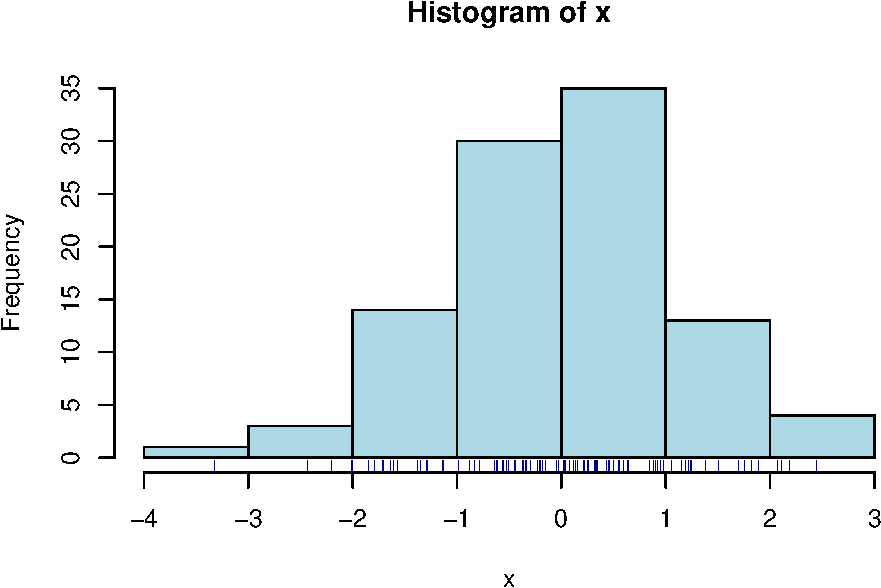
\includegraphics{bookdown-emlar2020_files/figure-latex/4.3.1-1.pdf}

\hypertarget{boxplot}{%
\section{\texorpdfstring{\texttt{boxplot}}{boxplot}}\label{boxplot}}

This yields a
boxplot summary \citep{tukey77} of one variable. You can also specify the
dependent and independent variable, with argument
\texttt{dv\textasciitilde{}iv1}; this will produce multiple
boxplots for the dependent variable, broken down by the independent
variable(s).
Two useful arguments for this command are:\\
\texttt{notch=T} to give additional information
about the distribution, and\\
\texttt{varwidth=T} to scale the width of the boxes
to the numbers of observations.

\begin{Shaded}
\begin{Highlighting}[]
\KeywordTok{boxplot}\NormalTok{( x, }\DataTypeTok{col=}\StringTok{"lightblue"}\NormalTok{, }\DataTypeTok{horizontal=}\OtherTok{TRUE}\NormalTok{, }\DataTypeTok{notch=}\OtherTok{TRUE}\NormalTok{, }\DataTypeTok{varwidth=}\OtherTok{TRUE}\NormalTok{ )}
\KeywordTok{rug}\NormalTok{(x, }\DataTypeTok{col=}\StringTok{"darkblue"}\NormalTok{ )}
\end{Highlighting}
\end{Shaded}

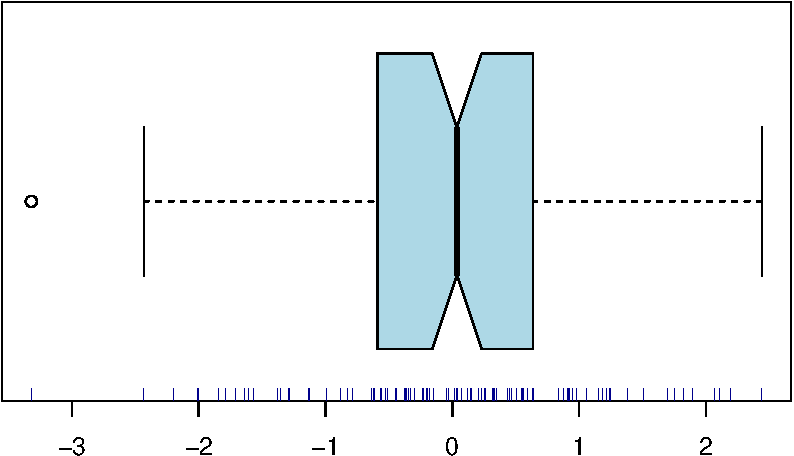
\includegraphics{bookdown-emlar2020_files/figure-latex/4.4.1-1.pdf}

\hypertarget{qqnorm}{%
\section{\texorpdfstring{\texttt{qqnorm}}{qqnorm}}\label{qqnorm}}

This produces a quantile--quantile (QQ) plot. This plots the
observed quantiles against the expected quantiles \emph{if} the argument
variable would be distributed normally. If the variable is indeed
distributed normally, then the data should fall on an approximately
straight line. Deviations of this line indicate deviations from
normality. You can also add the expected line with
{\texttt{qqline}}.

\hypertarget{summary-1}{%
\section{\texorpdfstring{\texttt{summary}}{summary}}\label{summary-1}}

This command produces a numerical summary of the argument variable.
However it does not supply standard measures of variability. We
often need

\hypertarget{var}{%
\section{\texorpdfstring{\texttt{var}}{var}}\label{var}}

to compute the variance of the argument variable. Related functions
are \texttt{sd} to compute standard deviation,
\texttt{cov} to compute the covariance between two
variables, and \texttt{cor} to compute their
correlation.

\hypertarget{length}{%
\section{\texorpdfstring{\texttt{length}}{length}}\label{length}}

returns the length of the argument variable, i.e.~the number of
observations in that vector. This is useful for checking the number
of data, as a preliminary for further analyses.

\begin{Shaded}
\begin{Highlighting}[]
\NormalTok{valid.n <-}\StringTok{ }\ControlFlowTok{function}\NormalTok{(x) \{ }
  \KeywordTok{length}\NormalTok{(x)}\OperatorTok{-}\KeywordTok{length}\NormalTok{(}\KeywordTok{which}\NormalTok{(}\KeywordTok{is.na}\NormalTok{(x))) }
\NormalTok{  \}}
\end{Highlighting}
\end{Shaded}

In the last command above, we have programmed a new function
\texttt{valid.n}, using standard functions provided
with R.

\hypertarget{unique}{%
\section{\texorpdfstring{\texttt{unique}}{unique}}\label{unique}}

returns a vector containing the (unsorted) unique values of the
argument variable, without duplicates. This is also useful for
checking your data.

\begin{Shaded}
\begin{Highlighting}[]
\NormalTok{x <-}\StringTok{ }\KeywordTok{c}\NormalTok{(}\DecValTok{3}\NormalTok{,}\DecValTok{3}\NormalTok{,}\DecValTok{3}\NormalTok{,}\DecValTok{1}\NormalTok{,}\DecValTok{1}\NormalTok{,}\DecValTok{2}\NormalTok{); }\KeywordTok{unique}\NormalTok{(x); }\KeywordTok{sort}\NormalTok{(}\KeywordTok{unique}\NormalTok{(x))}
\end{Highlighting}
\end{Shaded}

\begin{verbatim}
## [1] 3 1 2
\end{verbatim}

\begin{verbatim}
## [1] 1 2 3
\end{verbatim}

\hypertarget{table}{%
\section{\texorpdfstring{\texttt{table}}{table}}\label{table}}

returns a frequency table, i.e.~reports the number of observations
for each (combination of) value(s) of one or more variables. This
again is helpful for checking your data, to inspect the numbers of
observations per cell (see also \ref{sec:subselection}).
Tables can be one-dimensional (see
example below) or multidimensional. It is also possible to make a
frequency table of a frequency table!

\begin{Shaded}
\begin{Highlighting}[]
\NormalTok{x <-}\StringTok{ }\KeywordTok{rep}\NormalTok{(}\DecValTok{1}\OperatorTok{:}\DecValTok{3}\NormalTok{,}\DataTypeTok{each=}\DecValTok{7}\NormalTok{); }\KeywordTok{table}\NormalTok{(x) }\CommentTok{# three cells, each 7 observations, N=21}
\end{Highlighting}
\end{Shaded}

\begin{verbatim}
## x
## 1 2 3 
## 7 7 7
\end{verbatim}

\begin{Shaded}
\begin{Highlighting}[]
\KeywordTok{table}\NormalTok{( }\KeywordTok{table}\NormalTok{(x) ) }\CommentTok{# ok: all three cells have 7 observations, N=21}
\end{Highlighting}
\end{Shaded}

\begin{verbatim}
## 
## 7 
## 3
\end{verbatim}

A useful trick: if all cells should have the
same number of observations, then the table-of-table should contain
a single number representing the number of \emph{cells}.

\begin{Shaded}
\begin{Highlighting}[]
\NormalTok{x[ }\KeywordTok{sample}\NormalTok{(}\DecValTok{1}\OperatorTok{:}\DecValTok{3}\OperatorTok{*}\DecValTok{7}\NormalTok{, }\DataTypeTok{size=}\DecValTok{2}\NormalTok{) ] <-}\StringTok{ }\OtherTok{NA} \CommentTok{# replace 2 out of 21 obs by NA}
\KeywordTok{table}\NormalTok{( }\KeywordTok{table}\NormalTok{(x) ) }\CommentTok{# not ok: not all three cells have 7 observations, N<21}
\end{Highlighting}
\end{Shaded}

\begin{verbatim}
## 
## 6 7 
## 2 1
\end{verbatim}

The \texttt{lattice} package (see Chapter \ref{ch:packages}) contains additional functions for higher-order data visualization:
\texttt{xyplot},
\texttt{histogram},
\texttt{densityplot},
\texttt{cloud},
and more. For more information, enter the command
\texttt{help(lattice)}.

\begin{center}\rule{0.5\linewidth}{0.5pt}\end{center}

Now that we have obtained some insightful figures, we might want to
include these in our documents. The best procedure in Rstudio is to go to the Plots tab in the lower right pane, and select \texttt{Export\ \textgreater{}\ Save\ as\ image...} or \texttt{Export\ \textgreater{}\ Save\ as\ PDF...}. Figures in PDF format (extension
\texttt{pdf}) are easy to include in LaTeX documents, and are best for
publication. Other formats (e.g. \texttt{png}) are easy to include
in LaTeX, MS Word and web documents.

\hypertarget{ch:testinghypotheses}{%
\chapter{Testing hypotheses}\label{ch:testinghypotheses}}

\hypertarget{formula}{%
\section{formula}\label{formula}}

When testing hypotheses, and building regression models, we need to
specify the relations between variables. This is done in
R by means of a \emph{formula}, which is needed in many
statistical functions. In general, such a formula consists of a
response variable, followed by the tilde symbol
{\texttt{\textasciitilde{}}}, followed by a list of independent
variables and/or factors \citep{wilk73}.
In this list, the colon
\texttt{:} indicates an interaction effect (instead
of the sequence operator), and the asterisk
\texttt{*} is shorthand for main effects plus
interactions (instead of the multiplication operator).
By default,
the intercept \texttt{\textasciitilde{}1} is included in the
formula, unless suppressed explicitly
(\texttt{-1}). We have already encountered such a formula
in the boxplot example above.

\begin{verbatim}
y ~ x1 + x2 # only main effects 
y ~ x1 * x2 # shorthand for x1 + x2 + (x1:x2) 
\end{verbatim}

Consult the help files for further information on how to specify
complex models.

\hypertarget{t-test}{%
\section{\texorpdfstring{\(t\) test}{t test}}\label{t-test}}

There are three ways to use the t test.

In a one-sample test, the mean is compared against an expected mean,
with

\begin{Shaded}
\begin{Highlighting}[]
\KeywordTok{t.test}\NormalTok{( x1, }\DataTypeTok{mu=}\FloatTok{0.80}\NormalTok{ )}
\end{Highlighting}
\end{Shaded}

\begin{verbatim}
## 
##  One Sample t-test
## 
## data:  x1
## t = 1.8691, df = 99, p-value = 0.06456
## alternative hypothesis: true mean is not equal to 0.8
## 95 percent confidence interval:
##  0.7878051 1.2082871
## sample estimates:
## mean of x 
## 0.9980461
\end{verbatim}

In a two-sample test with independent observations, we often compare
the same dependent variable, broken down by an independent
variable.

\begin{Shaded}
\begin{Highlighting}[]
\KeywordTok{t.test}\NormalTok{( y[x1}\OperatorTok{<}\KeywordTok{median}\NormalTok{(x1)], y[x1}\OperatorTok{>}\KeywordTok{median}\NormalTok{(x1)] ) }\CommentTok{# y split up by median of x1}
\end{Highlighting}
\end{Shaded}

\begin{verbatim}
## 
##  Welch Two Sample t-test
## 
## data:  y[x1 < median(x1)] and y[x1 > median(x1)]
## t = -3.3044, df = 94.766, p-value = 0.001345
## alternative hypothesis: true difference in means is not equal to 0
## 95 percent confidence interval:
##  -1.0476023 -0.2612324
## sample estimates:
## mean of x mean of y 
##  2.749787  3.404204
\end{verbatim}

This could also be achieved by specifying the dependent and
independent variables in a formula:\\

\begin{Shaded}
\begin{Highlighting}[]
\KeywordTok{t.test}\NormalTok{( y }\OperatorTok{~}\StringTok{ }\NormalTok{(x1}\OperatorTok{<}\KeywordTok{median}\NormalTok{(x1)) ) }\CommentTok{# equivalent}
\end{Highlighting}
\end{Shaded}

\begin{verbatim}
## 
##  Welch Two Sample t-test
## 
## data:  y by x1 < median(x1)
## t = 3.3044, df = 94.766, p-value = 0.001345
## alternative hypothesis: true difference in means is not equal to 0
## 95 percent confidence interval:
##  0.2612324 1.0476023
## sample estimates:
## mean in group FALSE  mean in group TRUE 
##            3.404204            2.749787
\end{verbatim}

In a two-sample test with paired observations, we often compare two
different observations, stored in two different variables.

\begin{Shaded}
\begin{Highlighting}[]
\KeywordTok{t.test}\NormalTok{( x1, x2 )}
\end{Highlighting}
\end{Shaded}

\begin{verbatim}
## 
##  Welch Two Sample t-test
## 
## data:  x1 and x2
## t = -6.3729, df = 197.68, p-value = 1.279e-09
## alternative hypothesis: true difference in means is not equal to 0
## 95 percent confidence interval:
##  -1.2764242 -0.6731481
## sample estimates:
## mean of x mean of y 
## 0.9980461 1.9728323
\end{verbatim}

Note that the number of observations in the test (and hence d.f.)
varies in these examples.

\hypertarget{chisq.test}{%
\section{\texorpdfstring{\texttt{chisq.test}}{chisq.test}}\label{chisq.test}}

First, let us create two categorical variables, derived from a
speaker's \texttt{age} (in years) and average \texttt{phraselength} (in
syllables), for 80 speakers in the Corpus of Spoken Dutch (\texttt{talkers} data set; \citep{R-hqmisc}).
Categorical variables are created here with the
\texttt{cut} function, to create
\texttt{breaks=2} categories of \texttt{age} (young and
old) and of \texttt{phraselength} (short and long).

\begin{Shaded}
\begin{Highlighting}[]
\KeywordTok{require}\NormalTok{(hqmisc)}
\KeywordTok{data}\NormalTok{(talkers)}
\NormalTok{age.cat <-}\StringTok{ }\KeywordTok{cut}\NormalTok{( talkers}\OperatorTok{$}\NormalTok{age, }\DataTypeTok{breaks=}\DecValTok{2}\NormalTok{ )}
\NormalTok{phraselength.cat <-}\StringTok{ }\KeywordTok{cut}\NormalTok{( talkers}\OperatorTok{$}\NormalTok{nsyl, }\DataTypeTok{breaks=}\DecValTok{2}\NormalTok{ )}
\end{Highlighting}
\end{Shaded}

The hypothesis under study is that older speakers tend to produce
shorter phrases. This hypothesis may be tested with a \(\chi^2\) (chi
square) test.\\

\begin{Shaded}
\begin{Highlighting}[]
\KeywordTok{table}\NormalTok{( age.cat, phraselength.cat ) }\CommentTok{# show 2x2 table}
\end{Highlighting}
\end{Shaded}

\begin{verbatim}
##          phraselength.cat
## age.cat   (4.44,9] (9,13.6]
##   (21,40]       28       12
##   (40,59]       32        8
\end{verbatim}

\begin{Shaded}
\begin{Highlighting}[]
\KeywordTok{chisq.test}\NormalTok{( age.cat, phraselength.cat ) }
\end{Highlighting}
\end{Shaded}

\begin{verbatim}
## 
##  Pearson's Chi-squared test with Yates' continuity correction
## 
## data:  age.cat and phraselength.cat
## X-squared = 0.6, df = 1, p-value = 0.4386
\end{verbatim}

The data in the table show that, as hypothesized, the odds of older talkers producing short phrases (\(32/8\) or \(4.0:1\)) are indeed higher than the odds of younger talkers producing short phrases (\(28/12\) or \(2.3:1\)). The effect is far from significant, however, and \(H_0\) is not rejected.

\hypertarget{aov}{%
\section{\texorpdfstring{\texttt{aov}}{aov}}\label{aov}}

This function performs a between-subjects analysis of variance, with
only fixed factors \citep{john08} (For more complex
analyses of variance having repeated measures, see Johnson 2008; for mixed effects models, see Chapter \ref{ch:mixedeffects} and references cited there.)
In the example below we create a
response variable \texttt{aa} which is not normally distributed
(check
with \texttt{hist}, \texttt{qqnorm}, etc).\\

\begin{Shaded}
\begin{Highlighting}[]
\NormalTok{a1<-}\KeywordTok{rpois}\NormalTok{(}\DecValTok{20}\NormalTok{,}\DataTypeTok{lambda=}\DecValTok{2}\NormalTok{); a2<-}\KeywordTok{rpois}\NormalTok{(}\DecValTok{20}\NormalTok{,}\DataTypeTok{lambda=}\DecValTok{4}\NormalTok{); a3<-}\KeywordTok{rpois}\NormalTok{(}\DecValTok{20}\NormalTok{,}\DataTypeTok{lambda=}\DecValTok{6}\NormalTok{) }
\NormalTok{aa <-}\StringTok{ }\KeywordTok{c}\NormalTok{(a1,a2,a3) }
\NormalTok{x1 <-}\StringTok{ }\KeywordTok{as.factor}\NormalTok{(}\KeywordTok{rep}\NormalTok{(}\DecValTok{1}\OperatorTok{:}\DecValTok{3}\NormalTok{,}\DataTypeTok{each=}\DecValTok{20}\NormalTok{)) }
\CommentTok{# x1 corresponds with the three different poisson distributions within aa}
\NormalTok{x2 <-}\StringTok{ }\KeywordTok{as.factor}\NormalTok{(}\KeywordTok{rep}\NormalTok{( }\KeywordTok{rep}\NormalTok{(}\DecValTok{1}\OperatorTok{:}\DecValTok{2}\NormalTok{,}\DataTypeTok{each=}\DecValTok{10}\NormalTok{), }\DecValTok{3}\NormalTok{)) }\CommentTok{# no effect expected}
\KeywordTok{summary}\NormalTok{( model1.aov <-}\StringTok{ }\KeywordTok{aov}\NormalTok{(aa}\OperatorTok{~}\NormalTok{x1}\OperatorTok{*}\NormalTok{x2) )}
\end{Highlighting}
\end{Shaded}

\begin{verbatim}
##             Df Sum Sq Mean Sq F value     Pr(>F)    
## x1           2 109.73   54.87  15.512 0.00000475 ***
## x2           1   0.27    0.27   0.075      0.785    
## x1:x2        2   6.93    3.47   0.980      0.382    
## Residuals   54 191.00    3.54                       
## ---
## Signif. codes:  0 '***' 0.001 '**' 0.01 '*' 0.05 '.' 0.1 ' ' 1
\end{verbatim}

\hypertarget{ch:regression}{%
\chapter{Regression}\label{ch:regression}}

\hypertarget{lm}{%
\section{\texorpdfstring{\texttt{lm}}{lm}}\label{lm}}

This function is used for regression according to a linear model,
i.e.~linear regression. It returns a model-class object. There are
specialized functions for such models, e.g.
to extract residuals (\texttt{resid}),
to extract regression coefficients (\texttt{coef}),
to modify (\texttt{update}) the model, etc.

In the following example, we construct two regression models.
The first step in your regression analysis should always be a thorough visual and numerical inspection, including histograms and scatterplots of the variables under
study.

The first model is

\(\texttt{nsyl} = b_0\)

having only a
constant intercept. The second model includes the speakers' age as a
predictor, i.e.

\(\texttt{nsyl} = b_0 + b_1 \texttt{age}\)

(The intercept is included in this model too, by default, unless
suppressed explicitly with \texttt{-1} or
\texttt{\textasciitilde{}0} in the regression formula). The key
question here is whether inclusion of a predictor yields a better
model, with significantly smaller residuals and significantly higher
\(R^2\). The intercept-only model and the linear-regression model are
compared with the \texttt{anova} function.

\begin{Shaded}
\begin{Highlighting}[]
\KeywordTok{require}\NormalTok{(hqmisc)}
\KeywordTok{data}\NormalTok{(talkers)}
\NormalTok{model1.lm <-}\StringTok{ }\KeywordTok{lm}\NormalTok{( nsyl}\OperatorTok{~}\DecValTok{1}\NormalTok{, }\DataTypeTok{data=}\NormalTok{talkers ) }\CommentTok{# only intercept}
\NormalTok{model2.lm <-}\StringTok{ }\KeywordTok{lm}\NormalTok{( nsyl}\OperatorTok{~}\NormalTok{age, }\DataTypeTok{data=}\NormalTok{talkers ) }\CommentTok{# with intercept}
\KeywordTok{anova}\NormalTok{( model1.lm, model2.lm ) }\CommentTok{# compare two models}
\end{Highlighting}
\end{Shaded}

\begin{verbatim}
## Analysis of Variance Table
## 
## Model 1: nsyl ~ 1
## Model 2: nsyl ~ age
##   Res.Df    RSS Df Sum of Sq      F Pr(>F)
## 1     79 381.85                           
## 2     78 375.06  1    6.7823 1.4105 0.2386
\end{verbatim}

Including the \texttt{age} predictor does improve the model a little bit,
as indicated by the somewhat smaller residual sums-of-squares
(\texttt{RSS}). The improvement, however, is too small to be of
significance. The linear effect of a speaker's age on his or her
average phrase length (in syllables) is not significant.

\hypertarget{glm}{%
\section{\texorpdfstring{\texttt{glm}}{glm}}\label{glm}}

For logistic regression we use function
\texttt{glm(family=binomial)}, again with a
regression formula as an obligatory argument. Logistic regression
can be imagined as computing the logit of the hit-rate for each
cell, and then regressing these logits on the predictor(s). Here is
an annotated example \citep{MMC03} (Exercise 15.25).

The response variable \texttt{outcome} indicates
the death (\texttt{0}) or survival
(\texttt{1}) of 2900 patients in two hospitals.

\begin{Shaded}
\begin{Highlighting}[]
\NormalTok{ips1525 <-}\StringTok{ }\KeywordTok{read.table}\NormalTok{( }
  \DataTypeTok{file=}\KeywordTok{url}\NormalTok{(}\StringTok{"http://www.hugoquene.nl/emlar/ipsex1525.txt"}\NormalTok{),}
  \DataTypeTok{header=}\NormalTok{T, }\DataTypeTok{sep=}\StringTok{","}\NormalTok{) }
\KeywordTok{with}\NormalTok{( ips1525, }\KeywordTok{table}\NormalTok{(outcome) ) }
\end{Highlighting}
\end{Shaded}

\begin{verbatim}
## outcome
##    0    1 
##   79 2821
\end{verbatim}

\begin{Shaded}
\begin{Highlighting}[]
\KeywordTok{log}\NormalTok{(}\DecValTok{2821}\OperatorTok{/}\DecValTok{79}\NormalTok{) }\CommentTok{# log of odds of survival is 3.575}
\end{Highlighting}
\end{Shaded}

\begin{verbatim}
## [1] 3.575399
\end{verbatim}

\begin{Shaded}
\begin{Highlighting}[]
\CommentTok{# intercept-only logistic-regression model}
\NormalTok{model1.glm <-}\StringTok{ }\KeywordTok{glm}\NormalTok{( outcome}\OperatorTok{~}\DecValTok{1}\NormalTok{, }\DataTypeTok{data=}\NormalTok{ips1525, }\DataTypeTok{family=}\NormalTok{binomial )}
\KeywordTok{summary}\NormalTok{(model1.glm) }
\end{Highlighting}
\end{Shaded}

\begin{verbatim}
## 
## Call:
## glm(formula = outcome ~ 1, family = binomial, data = ips1525)
## 
## Deviance Residuals: 
##    Min      1Q  Median      3Q     Max  
## -2.684   0.235   0.235   0.235   0.235  
## 
## Coefficients:
##             Estimate Std. Error z value Pr(>|z|)    
## (Intercept)   3.5754     0.1141   31.34   <2e-16 ***
## ---
## Signif. codes:  0 '***' 0.001 '**' 0.01 '*' 0.05 '.' 0.1 ' ' 1
## 
## (Dispersion parameter for binomial family taken to be 1)
## 
##     Null deviance: 725.1  on 2899  degrees of freedom
## Residual deviance: 725.1  on 2899  degrees of freedom
## AIC: 727.1
## 
## Number of Fisher Scoring iterations: 6
\end{verbatim}

The intercept coefficient of the intercept-only logistic regression
model equals the overall log odds of survival; this intercept is
significantly different from zero \footnote{If the odds are \(1:1\), then the log of the odds is \(\log(1)=0\).}. Thus the intercept-only
logistic regression model captures the overall log odds of survival.
Next, let's try to improve this model, by including two predictors:
first, the \texttt{hospital} where the patient was treated, and second, the
patient's \texttt{condition} at intake, classified as bad
(\texttt{0}) or good (\texttt{1}).

\begin{Shaded}
\begin{Highlighting}[]
\NormalTok{model2.glm <-}\StringTok{ }\KeywordTok{glm}\NormalTok{( outcome}\OperatorTok{~}\NormalTok{hospital, }\DataTypeTok{data=}\NormalTok{ips1525, }\DataTypeTok{family=}\NormalTok{binomial ) }
\NormalTok{model3.glm <-}\StringTok{ }\KeywordTok{glm}\NormalTok{( outcome}\OperatorTok{~}\NormalTok{hospital}\OperatorTok{*}\NormalTok{condition, }
                   \DataTypeTok{data=}\NormalTok{ips1525, }\DataTypeTok{family=}\NormalTok{binomial ) }
\end{Highlighting}
\end{Shaded}

The deviance among logistic-regression models follows a \(\chi^2\)
distribution. Hence we can compare models by computing the \(\chi^2\)
probability of their deviances. Both model 2 and model 3
are compared here against model 1.

\begin{Shaded}
\begin{Highlighting}[]
\KeywordTok{anova}\NormalTok{( model1.glm, model2.glm, model3.glm, }\DataTypeTok{test=}\StringTok{"Chisq"}\NormalTok{ ) }
\end{Highlighting}
\end{Shaded}

\begin{verbatim}
## Analysis of Deviance Table
## 
## Model 1: outcome ~ 1
## Model 2: outcome ~ hospital
## Model 3: outcome ~ hospital * condition
##   Resid. Df Resid. Dev Df Deviance   Pr(>Chi)    
## 1      2899     725.10                           
## 2      2898     722.78  1   2.3253     0.1273    
## 3      2896     703.96  2  18.8222 0.00008181 ***
## ---
## Signif. codes:  0 '***' 0.001 '**' 0.01 '*' 0.05 '.' 0.1 ' ' 1
\end{verbatim}

The results indicate that there is no significant difference among
hospitals in their survival rates (model 2, \(p>.10\)), but there is a
significant effect of intake condition on the outcome (model 3,
\(p<.001\)). Of course, you should also inspect the models themselves
before drawing conclusions.

\hypertarget{ch:mixedeffects}{%
\chapter{Mixed-effects modeling}\label{ch:mixedeffects}}

Many language (acquisition) studies are based on samples of two random
factors: a sample of participants (subjects) and a sample of language
items (words, sentences, texts). The two random factors are \emph{crossed},
i.e., each item is presented to each participant --- often only once, so
that a subject does not respond to the same item repeatedly in multiple
conditions. The analysis methods shown above
(\texttt{aov}, \texttt{lm},
\texttt{glm}) all fail to acknowledge this particular
structure in the random part of the design. They include a single random
factor (named \texttt{Residual}) that aggregates all
random effects.

A better method is to use \emph{mixed-effects modeling},
which may be done in R by using the \texttt{lmer} command. Key
advantages of this method{[}\^{}15{]} are (a) it allows multiple random
factors, crossed and/or nested, (b) it does not require homogeneity of
variance, (c) it is robust against missing data. Hence mixed-effects
modeling is quickly gaining in popularity
\citep{QB04, QB08, baay08, HMS18}.

For mixed-effects modeling, you need to install two add-on packages to
R , named \texttt{lme4} and \texttt{languageR} \citep{BDB08}. For more
information on packages, see Chapter \ref{ch:packages} below.
After activation of these packages, we
can simply perform a mixed-effects analysis. First, we read in an
example dataset \citep{QB08} in long data layout:

\begin{Shaded}
\begin{Highlighting}[]
\NormalTok{x24 <-}\StringTok{ }\KeywordTok{read.table}\NormalTok{( }\DataTypeTok{file=}\KeywordTok{url}\NormalTok{(}\StringTok{"http://www.hugoquene.nl/emlar/x24r2.txt"}\NormalTok{), }\DataTypeTok{header=}\NormalTok{T )}
\end{Highlighting}
\end{Shaded}

These fictitious responses were provided by 24 subjects, for 36 items,
in 3 conditions, with rotation of items over conditions. This rotation
may be inspected for a small subset of the data frame:

\begin{Shaded}
\begin{Highlighting}[]
\KeywordTok{with}\NormalTok{( }\KeywordTok{subset}\NormalTok{(x24, subj}\OperatorTok{<=}\DecValTok{3}\OperatorTok{&}\NormalTok{item}\OperatorTok{<=}\DecValTok{6}\NormalTok{), }\KeywordTok{table}\NormalTok{(subj,item,cond) ) }
\end{Highlighting}
\end{Shaded}

\begin{verbatim}
## , , cond = 1
## 
##     item
## subj 1 2 3 4 5 6
##    1 1 1 1 1 1 1
##    2 0 0 0 0 0 0
##    3 0 0 0 0 0 0
## 
## , , cond = 2
## 
##     item
## subj 1 2 3 4 5 6
##    1 0 0 0 0 0 0
##    2 1 1 1 1 1 1
##    3 0 0 0 0 0 0
## 
## , , cond = 3
## 
##     item
## subj 1 2 3 4 5 6
##    1 0 0 0 0 0 0
##    2 0 0 0 0 0 0
##    3 1 1 1 1 1 1
\end{verbatim}

Next, we need to specify that \texttt{cond} is a
categorical factor, and not a continuous predictor. In addition, we
specify the levels of the factor, we specify its contrasts, and indicate
that the second level is the baseline or reference level.

\begin{Shaded}
\begin{Highlighting}[]
\NormalTok{x24}\OperatorTok{$}\NormalTok{cond <-}\StringTok{ }\KeywordTok{as.factor}\NormalTok{(x24}\OperatorTok{$}\NormalTok{cond)}
\KeywordTok{contrasts}\NormalTok{(x24}\OperatorTok{$}\NormalTok{cond) <-}\StringTok{ }\KeywordTok{contr.treatment}\NormalTok{( }\KeywordTok{c}\NormalTok{(}\StringTok{".A"}\NormalTok{,}\StringTok{".B"}\NormalTok{,}\StringTok{".C"}\NormalTok{), }\DataTypeTok{base=}\DecValTok{2}\NormalTok{ )}
\end{Highlighting}
\end{Shaded}

After these preliminary steps we can estimate an appropriate mixed-effects
model in a single command. The estimated model is also stored as an
object, and a summary is displayed.

\begin{Shaded}
\begin{Highlighting}[]
\KeywordTok{summary}\NormalTok{( x24.m1 <-}\StringTok{ }\KeywordTok{lmer}\NormalTok{(resp }\OperatorTok{~}\StringTok{ }\DecValTok{1}\OperatorTok{+}\NormalTok{cond}\OperatorTok{+}\NormalTok{(}\DecValTok{1}\OperatorTok{|}\NormalTok{subj)}\OperatorTok{+}\NormalTok{(}\DecValTok{1}\OperatorTok{|}\NormalTok{item),}
                        \DataTypeTok{data=}\NormalTok{x24, }\DataTypeTok{REML=}\OtherTok{FALSE}\NormalTok{) )}
\end{Highlighting}
\end{Shaded}

\begin{verbatim}
## Linear mixed model fit by maximum likelihood  ['lmerMod']
## Formula: resp ~ 1 + cond + (1 | subj) + (1 | item)
##    Data: x24
## 
##      AIC      BIC   logLik deviance df.resid 
##   2046.8   2075.4  -1017.4   2034.8      858 
## 
## Scaled residuals: 
##     Min      1Q  Median      3Q     Max 
## -3.1641 -0.6394 -0.0077  0.6416  2.7157 
## 
## Random effects:
##  Groups   Name        Variance Std.Dev.
##  item     (Intercept) 0.2579   0.5078  
##  subj     (Intercept) 0.2891   0.5377  
##  Residual             0.5103   0.7144  
## Number of obs: 864, groups:  item, 36; subj, 24
## 
## Fixed effects:
##             Estimate Std. Error t value
## (Intercept)  0.04569    0.14485   0.315
## cond.A       0.17037    0.05953   2.862
## cond.C      -0.23696    0.05953  -3.980
## 
## Correlation of Fixed Effects:
##        (Intr) cond.A
## cond.A -0.205       
## cond.C -0.205  0.500
\end{verbatim}

The output correctly shows that there are two unrelated random effects,
plus unexplained residual variance. Each response is now modeled as a
unique combination of the intercept (mean of baseline condition B), item
effect, subject effect, condition effect, and residual. The average
response in the baseline condition B is \(0.046\) units. Responses in
condition A are 0.170 units higher than baseline, and in condition C
they are \(-0.237\) units higher than baseline, i.e. \(0.237\) units lower.

For reasons not discussed here \footnote{See Frequently Asked Questions about R, Question
  7.35, at \url{http://cran.r-project.org/doc/FAQ/R-FAQ.html}}, the significance levels of the
fixed effects are not reported in the output of
\texttt{lmer}. There are several solutions to obtain
these significance levels.

\begin{itemize}
\tightlist
\item
  The most conservative option \citep{HMS18} is to use the critical \(t\) value
  associated with the random effect that has the fewest levels (here
  \texttt{subj}), corrected for the number of fixed
  coefficients including the intercept (here \(3\)).
  If a fixed effect is significant by this very
  conservative criterion, then it will also be significant by any other
  criterion that is less conservative and more liberal.
\end{itemize}

\begin{Shaded}
\begin{Highlighting}[]
\KeywordTok{qt}\NormalTok{( }\DataTypeTok{p=}\DecValTok{1}\FloatTok{-.05}\OperatorTok{/}\DecValTok{2}\NormalTok{, }\DataTypeTok{df=}\DecValTok{24-3}\NormalTok{ ) }\CommentTok{# critical value t*, alpha=.05, two-sided}
\end{Highlighting}
\end{Shaded}

\begin{verbatim}
## [1] 2.079614
\end{verbatim}

Comparison of the fixed effects with this critical \(t^*\) = 2.08 shows that
both conditions A and C differ significantly from the baseline condition
B.

\begin{itemize}
\tightlist
\item
  A second option is to estimate 95\% confidence intervals for all
  coefficients in the resulting mixed-effects model. This can be
  time-consuming, as the mixed-effects model will be re-fit many times on
  slightly varying datasets.
\end{itemize}

\begin{Shaded}
\begin{Highlighting}[]
\CommentTok{# warnings may occur}
\KeywordTok{print}\NormalTok{( x24.m1.ci <-}\StringTok{ }\KeywordTok{confint}\NormalTok{( x24.m1, }\DataTypeTok{method=}\StringTok{"boot"}\NormalTok{, }\DataTypeTok{nsim=}\DecValTok{250}\NormalTok{ ))}
\end{Highlighting}
\end{Shaded}

\begin{verbatim}
## Computing bootstrap confidence intervals ...
\end{verbatim}

\begin{verbatim}
## 
## 6 warning(s): Model failed to converge with max|grad| = 0.00267345 (tol = 0.002, component 1) (and others)
\end{verbatim}

\begin{verbatim}
##                   2.5 %     97.5 %
## .sig01       0.35950709  0.6747204
## .sig02       0.36333157  0.6844652
## .sigma       0.68054619  0.7474401
## (Intercept) -0.23533348  0.3634542
## cond.A       0.05695928  0.3035280
## cond.C      -0.36262503 -0.1261797
\end{verbatim}

As the interval for \texttt{cond.A} is entirely
positive, we may conclude with 95\% confidence that condition A yields
higher scores than the baseline condition B, and mutatis mutandis that
condition C yields lower scores than condition B.

\hypertarget{ch:packages}{%
\chapter{Packages}\label{ch:packages}}

Packages are user-provided extensions to the basic R
system (comparable to an ``add-on'' or ``extension'' for some web browsers).
Packages
may contain custom datasets, additional functions, re-formulations of
existing functions, and more. There are by now thousands of useful
packages extending R.

A package named \texttt{ABC} can be installed by
entering \texttt{install.packages("ABC")} (with double quotes) and then \texttt{require(ABC)} (without double quotes).
If a package in turn requires other packages, these are also installed
and loaded.

Some useful packages are the following:

\begin{itemize}
\item
  \texttt{datasets}: A wide
  variety of datasets, for exploration and education. This
  package is now integrated within R (see Help on \texttt{datasets}).
\item
  \texttt{foreign}: Functions for reading and writing data stored by statistical
  packages such as Minitab, S, SAS, SPSS, Stata, Systat, and for
  reading CSV files (comma separated values) created by Microsoft
  Excel, and for reading and writing dBase files \citep{R-foreign}.
\item
  \texttt{lattice}: Trellis graphics for R. The functions provide a
  powerful, elegant and flexible high-level data visualization system,
  using Trellis graphics, with an emphasis on multivariate data \citep{R-lattice}.
\item
  \texttt{MASS}: Datasets and functions accompanying \citep{VR02, R-MASS}
\item
  \texttt{languageR}: Datasets and functions accompanying \citep{baay08, R-languageR}.
\item
  \texttt{hqmisc}: Some convenience functions and an example dataset, by the present author \citep{R-hqmisc}, and used in this booklet.
\item
  \texttt{tidyverse}: A meta-package consisting of many other packages supporting your data science, such as \texttt{dplyr} for data transformation, \texttt{ggplot2} for data visualization, and \texttt{rmarkdown} for reporting (also used for this booklet) \citep{tidy19}; all component packages can also be used separately.
\end{itemize}

Packages are stored on a so-called \emph{repository}; the CRAN repository is
the most important one (\url{https://cran.r-project.org/}).
You should use a nearby mirror site of the CRAN
repository, by giving the command \texttt{chooseCRANmirror()}.
Rstudio and R remember your chosen mirror site over multiple sessions.

Finally, to inspect the status of your current session in R, use the command \texttt{sessionInfo()}. This will return a listing of technical information, locale settings, all attached packages, and all loaded packages, with version info for each.

\hypertarget{sec:furtherreading}{%
\chapter{Further reading}\label{sec:furtherreading}}

A wealth of useful documentation is available through the \texttt{Help} tab
in the lower right pane of RStudio. Browse in the FAQ files, the help files, the
manuals and the vignettes that come with R and Rstudio.

More help can be called from within R by giving the command
\texttt{help(ABC)} or \texttt{?ABC} with a
command or operator as argument.
(This can be typed in the \texttt{Console} tab in the lower left pane of RStudio.)

There is also a lot more help available on the internet, in particular
from the R project website \url{https://www.r-project.org}
and the RStudio website \url{https://www.Rstudio.com}.

A few other useful web resources are:

\begin{itemize}
\item
  Quick-R, \url{http://statmethods.net}
\item
  \url{http://math.illinoisstate.edu/dhkim/Rstuff/Rtutor.html}
\end{itemize}

The following three books on using R and on its
applications in linguistics are highly recommended:
\citep{baay08, john08, adler10}.

Happy analyses!

\bibliography{book.bib,packages.bib,emlar.bib}

\end{document}
